\documentclass[a4paper,10 pt]{article} 
\usepackage[french,italian]{babel} 
\usepackage[T1]{fontenc} 
\usepackage[utf8]{inputenc}                             
\usepackage{graphicx}
\usepackage[normalem]{ulem}
\useunder{\uline}{\ul}{}
\usepackage[a4paper, top=2cm, bottom=3cm, left=1.7cm, right=1.7cm]{geometry}
\usepackage{booktabs}
\usepackage{array}
\usepackage{quoting}
\usepackage{physics}
\usepackage{amsmath}
\usepackage{tikz}
\usepackage{mathdots}
\usepackage{yhmath}
\usepackage{cancel}
\usepackage{color}
\usepackage{siunitx}
\usepackage{array}
\usepackage{multirow}
\usepackage{amssymb}
\usepackage{gensymb}
\usepackage{tabularx}
\usepackage{booktabs}
\usetikzlibrary{fadings}
\usetikzlibrary{patterns}
\usetikzlibrary{shadows.blur}
\usetikzlibrary{shapes}
\usepackage{subfig}
\usepackage[colorlinks]{hyperref}
% Per creare un "blocco" codice
\usepackage{xcolor}
\usepackage{listings}

\colorlet{mygray}{black!30}
\colorlet{mygreen}{green!60!blue}
\colorlet{mymauve}{red!60!blue}

\lstset{
  backgroundcolor=\color{gray!10},  
  basicstyle=\ttfamily,
  columns=fullflexible,
  breakatwhitespace=false,      
  breaklines=true,                
  captionpos=b,                    
  commentstyle=\color{mygreen}, 
  extendedchars=true,              
  frame=single,                   
  keepspaces=true,             
  keywordstyle=\color{blue},      
  language=c++,                 
  numbers=none,                
  numbersep=5pt,                   
  numberstyle=\tiny\color{blue}, 
  rulecolor=\color{mygray},        
  showspaces=false,               
  showtabs=false,                 
  stepnumber=5,                  
  stringstyle=\color{mymauve},    
  tabsize=3,                      
  title=\lstname                
} % fine

\title{Laboratorio di Programmazione C++/ROOT:
\
\\
Simulazione di un Esperimento di Fisica Nucleare} 
\author{Lanzi Samuele}
\date{A.A. 2020-2021}

\begin{document}

\maketitle

\section{Introduzone}
Questo programma ha lo scopo di implementare un prototipo di codice utilizzabile per rappresentare 
e analizzare il contenuto di eventi fisici simulati risultanti da collisioni di particelle elementari.
Ognuno dei $\sim 10^5$ eventi che andiamo ad analizzare consite di $\sim 10^2$ particelle di tipi diversi, 
con aggiunta delle risonanze; ciascun tipo possiede una certa abbondanza (una certa probabilità di essere generato).

\
\\
Parleremo della struttura del programma scritto in C++ con l'ausilio di ROOT nella sezione 2 per poi passare alla 
generazione degli eventi nella sezione 3, successivamente analizzeremo quanto ottenuto nella sezione 4.

\section{Struttura del Codice}
Il programma è basato su 3 classi due delle quali sfruttano il polimorfismo dinamico grazie 
al quale una classe figlia può ereditare alcune caratteristiche della classe madre.
\begin{itemize}
    \item[-] {\bf ParticleType} descrittiva di alcune proprietà di base delle particelle elementari avente come 
    attributi privati il nome \verb!fName!, la massa \verb!fMass! e la carica \verb!fCharge! della particella; 
    come metodi abbiamo i getters per gli attributi, un metodo \verb!Print()! per stampare a schermo 
    le proprietà della particella ed un costruttore parametrico.

    \item[-] {\bf ResonanceType} descrittiva di alcune proprietà di base specifiche delle risonanze, che erdita 
    da \verb!ParticleType! ed ha come attributo aggiuntivo privato la larghezza della risonanza \verb!fWidth! e 
    come metodi pubblici un costruttore parametrico ed un metodo \verb!Print()! che eredita quello della classe madre ed aggiunge un attributo 
    da stampare.

    \item[-] {\bf Particle} descrittiva sia delle proprietà di base definite nella classe \verb!ParticleType! e nella
    sua derivata che delle proprietà cinematiche (le tre componenti dell'impulso) di una particella. La classe ha come attributi
    privati: un costruttore parametrico;
    un \verb!static std::vector<ParticleType*> fParticleType! che contiene le informazioni dei tipi di particelle
    che saranno generati nel \verb!main!; una varibile interna \verb!fIParticle! che rappresenta l'indice dell'
    elemento del vettore di puntatori; le tre componenti dell'impulso raggruppate in un nuovo tipo di dato \verb!P fP! \footnote{Per ulteriori dettagli consultare l'Appendice 1}. 
    Come metodi pubblici abbiamo i getter, un metodo statico per fare il \verb!push! di elementi nel vettore ed altri metodi per ricavare grandezze a partire
    dall'impulso e dalla massa: \verb!Energy()! per l'energia, \verb!invMass()! per la massa invariante $\dots$
\end{itemize} \begin{figure}[h]
\centering
\tikzset{every picture/.style={line width=0.75pt}} %set default line width to 0.75pt        
\begin{tikzpicture}[x=0.75pt,y=0.75pt,yscale=-0.85,xscale=0.85]
%uncomment if require: \path (0,300); %set diagram left start at 0, and has height of 300
%Rounded Rect [id:dp20615820737265156] 
\draw   (116.5,151) .. controls (116.5,146.58) and (120.08,143) .. (124.5,143) -- (248.5,143) .. controls (252.92,143) and (256.5,146.58) .. (256.5,151) -- (256.5,176) .. controls (256.5,180.42) and (252.92,184) .. (248.5,184) -- (124.5,184) .. controls (120.08,184) and (116.5,180.42) .. (116.5,176) -- cycle ;
%Shape: Rectangle [id:dp4661821073560425] 
\draw   (91.5,48) -- (280.5,48) -- (280.5,195) -- (91.5,195) -- cycle ;
%Rounded Rect [id:dp15238098637275865] 
\draw   (116.5,69) .. controls (116.5,64.58) and (120.08,61) .. (124.5,61) -- (248.5,61) .. controls (252.92,61) and (256.5,64.58) .. (256.5,69) -- (256.5,94) .. controls (256.5,98.42) and (252.92,102) .. (248.5,102) -- (124.5,102) .. controls (120.08,102) and (116.5,98.42) .. (116.5,94) -- cycle ;
%Rounded Rect [id:dp40566555480564326] 
\draw   (330.5,115) .. controls (330.5,110.58) and (334.08,107) .. (338.5,107) -- (462.5,107) .. controls (466.92,107) and (470.5,110.58) .. (470.5,115) -- (470.5,140) .. controls (470.5,144.42) and (466.92,148) .. (462.5,148) -- (338.5,148) .. controls (334.08,148) and (330.5,144.42) .. (330.5,140) -- cycle ;
%Straight Lines [id:da542247619427663] 
\draw    (185.93,140.15) -- (186.06,105.85) ;
\draw [shift={(186.07,102.85)}, rotate = 450.22] [fill={rgb, 255:red, 0; green, 0; blue, 0 }  ][line width=0.08]  [draw opacity=0] (8.93,-4.29) -- (0,0) -- (8.93,4.29) -- cycle    ;
%Straight Lines [id:da009375194794216335] 
\draw    (280.84,128) -- (329.84,128) ;
\draw [shift={(329.84,128)}, rotate = 0] [color={rgb, 255:red, 0; green, 0; blue, 0 }  ][fill={rgb, 255:red, 0; green, 0; blue, 0 }  ][line width=0.75]      (0, 0) circle [x radius= 3.35, y radius= 3.35]   ;

% Text Node
\draw (130,154) node [anchor=north west][inner sep=0.75pt]   [align=center] {$ResonanceType$};
% Text Node
\draw (147,72) node [anchor=north west][inner sep=0.75pt]   [align=center] {$ParticleType$};
% Text Node
\draw (373,119) node [anchor=north west][inner sep=0.75pt]   [align=center] {$Particle$};

\end{tikzpicture}
\caption{Schema della struttura del codice, come si può vedere la classe Particle non erdita proprietà dalle altre due ma usa il meccanismo della composizione.}
\end{figure}

Essendo \verb!ResonanceType! un tipo specializzato di \verb!ParticleType! (relazione “{\bf is a}”), la scelta è stata quella di riutilizzare il codice scritto per \verb!ParticleType! e far ereditare 
\verb!ResonanceType! da \verb!ParticleType!. La classe \verb!Particle! è una classe ulteriormente specializzata, che contiene sia le informazioni delle proprietà di base (nome, massa, carica, eventualmente larghezza di risonanza),
sia le proprietà cinematche (impulso 3D). In questo caso specifico la soluzione migliore per implementare \verb!Particle! è usare la composizione (aggregazione) [Figura-1]; includiamo in \verb!Particle! un membro statico che fa da tabella 
per i tipi di particella e relative proprietà di base così da avere un grosso risparmio in memoria.

\section{Generazione}
Nella nostra simulazione sono stati generati $\sim 10^5$ eventi ciascuno da $\sim 10^2$ particelle. Le particelle generate 
sono di sette tipi diversi: pioni ($\pi^+$, $\pi^-$), kaoni ($K^+$, $K^-$), protoni ($p^+$, $p^-$) e risonanza ($K^*$) ogni tipo 
di particella ha caratteristiche diverse sintetizzate in [Tabella-1].
\begin{table}[h]
    \centering
    \begin{tabular}{|l|l|l|l|l|}
    \hline
    {\bf Tipo di Particella} & {\bf Probabilità} & {\bf Massa} ($GeV/c^2$) & {\bf Carica} & \begin{tabular}[c]{@{}l@{}}{\bf Larghezza della} \\ {\bf Risonanza} ($GeV/c^2$) \end{tabular} \\ \hline
    $\pi^+$            & 0.4         & 0.13957           & +1     & -                                     \\ \hline
    $\pi^-$            & 0.4         & 0.13957           & -1     & -                                     \\ \hline
    $K^+$              & 0.05        & 0.49367           & +1     & -                                     \\ \hline
    $K^-$              & 0.05        & 0.49367           & -1     & -                                     \\ \hline
    $p^+$              & 0.045       & 0.93827           & +1     & -                                     \\ \hline
    $p^-$              & 0.045       & 0.93827           & -1     & -                                     \\ \hline
    $K^*$              & 0.01        & 0.89166           & 0      & 0.050                                 \\ \hline
    \end{tabular}
    \caption{Tipi di particelle e le loro caratteristiche}
\end{table} Alcune delle $100$ particelle generate in un evento, quindi, possono essere dello stesso tipo ma ciò che le 
contraddistingue le une dalle altre è l'impulso. Per settare le componenti dell'impulso procediamo, in prima battuta, a generarne il modulo casualmente
tramite il metodo Monte Carlo chiamato \verb!TRandom::Exp(1)!; successivamente possiamo risalire alle
componenti 3D (in coordinate sferiche) grazie alle seguenti:
\[
    \vec P = (P_x, P_y, P_z) \ \ conosciamo \ |\vec P| \equiv P
\]
\begin{equation}
    P_x = P \sin \theta \cos \phi \ \ \ \theta \in [0, \pi] \ e \ \phi \in [0, 2\pi]
\end{equation}
\[
 P_y = P \sin \theta \sin \phi
\]
\[
    P_z = P \cos \theta
\] Gli angoli $\theta$ (angolo polare) e $\phi$ (angolo azimutale) sono anch'essi generati casualmente attraverso il metodo di generazione Monte Carlo
\verb!TRandom::Uniform()!.

\
\\
Una volta generate tutte le particelle, quelle di tipo $K^*$ vengono fatte decadere in due coppie (ogni coppia ha il $50\%$ di probabilità di essere creata)
$(\pi^+, K^-)$ oppure $(\pi^-, K^+)$; all'interno del programma il decadimento avviene attraverso il metodo \verb!Particle::Decay2Body()!.

\section{Analisi}
\subsection{Abbondanza di Particelle, Angoli ed Impulso}
Analizziamo ora ciò che è emerso dal nostro programma iniziando dall'abbondanza di tipi di particelle 
riportata in [Tabella-2]. Come si può vedere i valori ricavati dal programma sono del tutto compatibili 
con i valori di aspettazione nel limite di errori statistici. In [Figura-2] è riportato l'istogramma nel 
quale ogni bin rappresenta un tipo di particella.

\begin{table}[h]
    \centering
    \begin{tabular}{|l|l|l|}
    \hline
    {\bf Specie}  & {\bf Occorrenze Osservate} & {\bf Occorrenze attese} \\ \hline
    $\pi^+$ & $(3999.3 \pm 2.0) \cdot 10^3$ & $4000 \cdot 10^3$ \\ \hline
    $\pi^-$ & $(4002.1 \pm 2.0) \cdot 10^3$ & $4000 \cdot 10^3$ \\ \hline
    $K^+$   & $(499.50 \pm 0.71) \cdot 10^3$ & $500 \cdot 10^3$ \\ \hline
    $K^-$   & $(498.69 \pm 0.71) \cdot 10^3$ & $500 \cdot 10^3$ \\ \hline
    $p^+$   & $(450.17 \pm 0.67) \cdot 10^3$ & $450 \cdot 10^3$ \\ \hline
    $p^-$   & $(450.48 \pm 0.67) \cdot 10^3$ & $450 \cdot 10^3$ \\ \hline
    $K^*$   & $(99.74 \pm 0.32) \cdot 10^3$ & $100 \cdot 10^3$ \\ \hline
    \end{tabular}
    \caption{Abbondanza dei tipi di particelle}
\end{table} 
Procediamo con gli istogrammi degli angoli azimutali e polari, come possiamo intuire dalla [Figura-2] i due istogrammi
seguono una distribuzione uniforme individuata dalla linea rossa; in [Tabella-3] sono riportati i valori del $\chi^2$ grazie
ai quali possiamo concludere che effettivamente il fit è consistente con la distribuzione generata. Consideriamo ora l'istogramma che rappresenta
il modulo dell'impuso [Figura-2] anch'esso fittato con una distribuzione, questa volta esponenziale, la quale è in perfetto accordo con quanto ci 
aspettavamo a meno di fluttuazioni statistiche.

\begin{table}[h]
    \centering
    \begin{tabular}{|l|l|l|l|l|}
    \hline
    {\bf Distribuzione} & {\bf Parametri del Fit} & $\chi^2$ & $\nu$ & $\chi^2/\nu$ \\ \hline
    Fit a distribuzione angolo $\theta$ (rad) & $100000 \pm 32$ & $98.75$ & 99 & 0.99 \\ \hline
    Fit a distribuzione angolo $\phi$ (rad) & $100000 \pm 32$ &  $99.04$ & 99 & 1.00  \\ \hline
    Fit a distribuzione modulo impulso ($GeV/c$) & $-1 \pm 0.0$ & 60.43 & 78 &  0.78\\ \hline
    \end{tabular}
    \caption{Distribuzioni dell'angolo azimutale, polare e dell'impulso}
\end{table}

\begin{figure}[h]
    \centering
    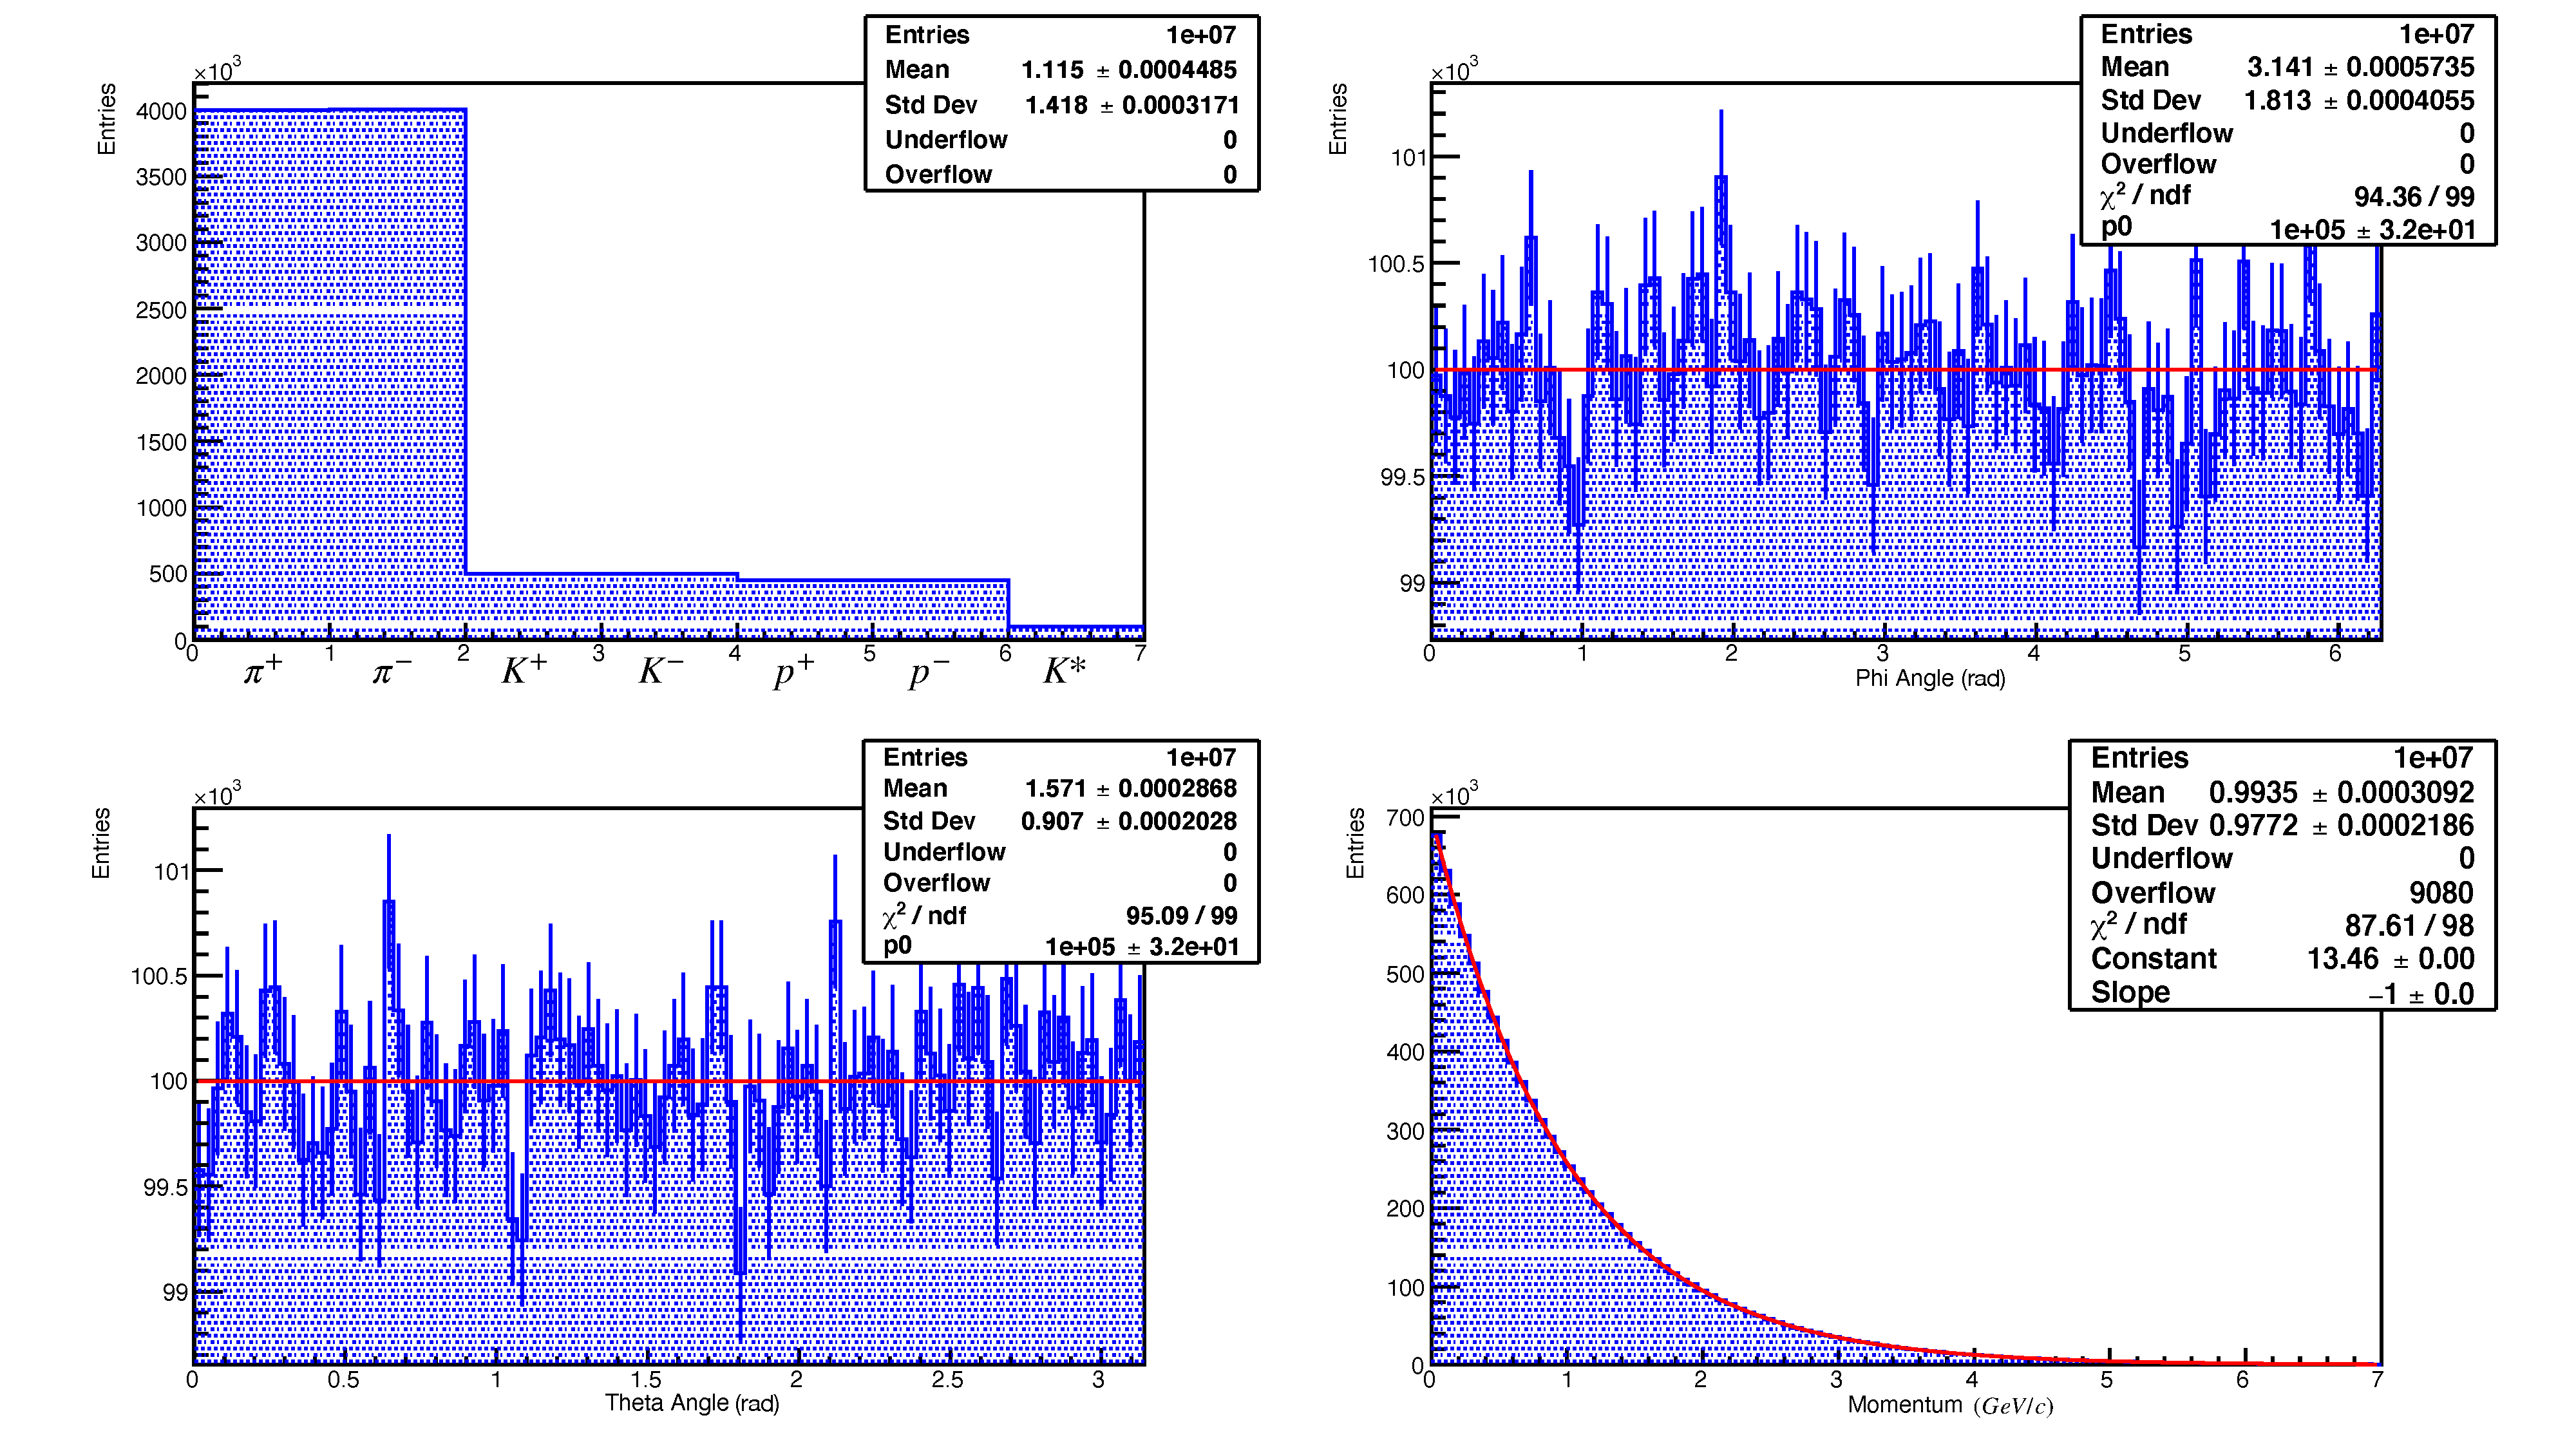
\includegraphics[scale=0.25]{c1.pdf}
    \caption{In alto a sinistra è rappresentato l'istogramma dell'abbondanza di particelle i cui valori
    precisi sono riportati in Tabella 1; in alto a destra e in basso a sinistra sono riportati gli 
    istogrammi dell'angolo azimutale e dell'angolo polare (fittati opportunamente con una distribuzione uniforme); in basso a destra è riportato l'istogramma
    dell'impulso (fittato con un esponenziale).}
\end{figure}

\subsection{Massa Invariante}
Passiamo ora agli istogrammi delle masse invarianti. Come avevamo accennato attraverso un metodo specifico le
particelle di tipo $K^*$ vengono fatte decadere in $(\pi^+, K^-)$ oppure $(\pi^-, K^+)$, se misuriamo le 
masse invarianti (attraverso il metodo \verb!invMass()!) tra tutte le particelle prodotte da questo decadimento 
in tutti gli eventi otteniamo il primo istogramma (di controllo) della [Figura-3] il quale è stato opportunamente fittato con una
gaussiana (le specifiche sono riportate in [Tabella-4]). 

\ 
\\
Per ricavare il secondo istogramma si può procedere in due step:
\begin{itemize}
    \item[-] Selezionando tra tutte quelle generate in un singolo evento le coppie di particelle
    del tipo $(\pi^+, K^-)$ e $(\pi^-, K^+)$, ricavandone a due a due la massa invariante e facendone un primo
    istogramma (1); ripetendo lo stesso procedimento per $(\pi^+, K^+)$ e $(\pi^-, K^-)$ si ottiene un secondo 
    istogramma (2);
    \item[-] Facendo ora la differenza tra i due istogrammi ottenuti (2) - (1) otteniamo il nostro risultato 
    riportato in [Figura-3]; fittandolo opportunamente con una gaussiana è inconfutabile la somiglianza con la distribuzione 
    ricavata in precedenza.
\end{itemize}

\ 
\\ 
Per ottenere il terzo istogramma il procedimento è molto simile a quello precedente con l'unica differenza che
invece di considerare le sole $\pi K$ con segni discordi e concordi si considerano le masse invarianti tra coppie di
particelle di qualsiasi tipo aventi comunque cariche di segno concorde e discorde. 

\ 
\\
Analizzando i risultati [Tabella-4] possiamo concludere che a meno di errori statistici ciò che abbiamo ottenuto è
consistente con quanto ipotizzato, ne sono un riprova i valori congrui del $\chi^2$. 
\begin{table}[h]
    \centering
    \begin{tabular}{|l|l|l|l|l|}
    \hline
    {\bf Distribuzione}                                                                                                                                & {\bf Media} (GeV/$c^2$) & {\bf Sigma} (GeV/$c^2$)& {\bf Ampiezza} & $\chi^2/\nu$ \\ \hline
    Massa Invariante vere $K^*$                                                                                                                    & $0.8914 \pm 0.0002$ & $0.05003 \pm 0.00011$ & $10020 \pm 39$ & $0.77$ \\ \hline
    \begin{tabular}[c]{@{}l@{}}Massa Invariante ottenuta da \\ differenza delle combinazioni \\ $\pi K$ di carica discorde e concorde\end{tabular} & $0.891 \pm 0.003$ & $0.050 \pm 0.003$ & $10580 \pm 490$&  $1.04$\\ \hline
    \begin{tabular}[c]{@{}l@{}}Massa Invariante ottenuta da \\ differenza delle combinazioni \\ di carica discorde e concorde\end{tabular}  & $0.895 \pm 0.005$ & $0.049 \pm 0.005$ & $9666 \pm 820$ & $1.05$\\ \hline
    \end{tabular}
    \caption{Masse invarianti di particelle opportunamente raggruppate}
\end{table}

\begin{figure}[!]
    \centering
    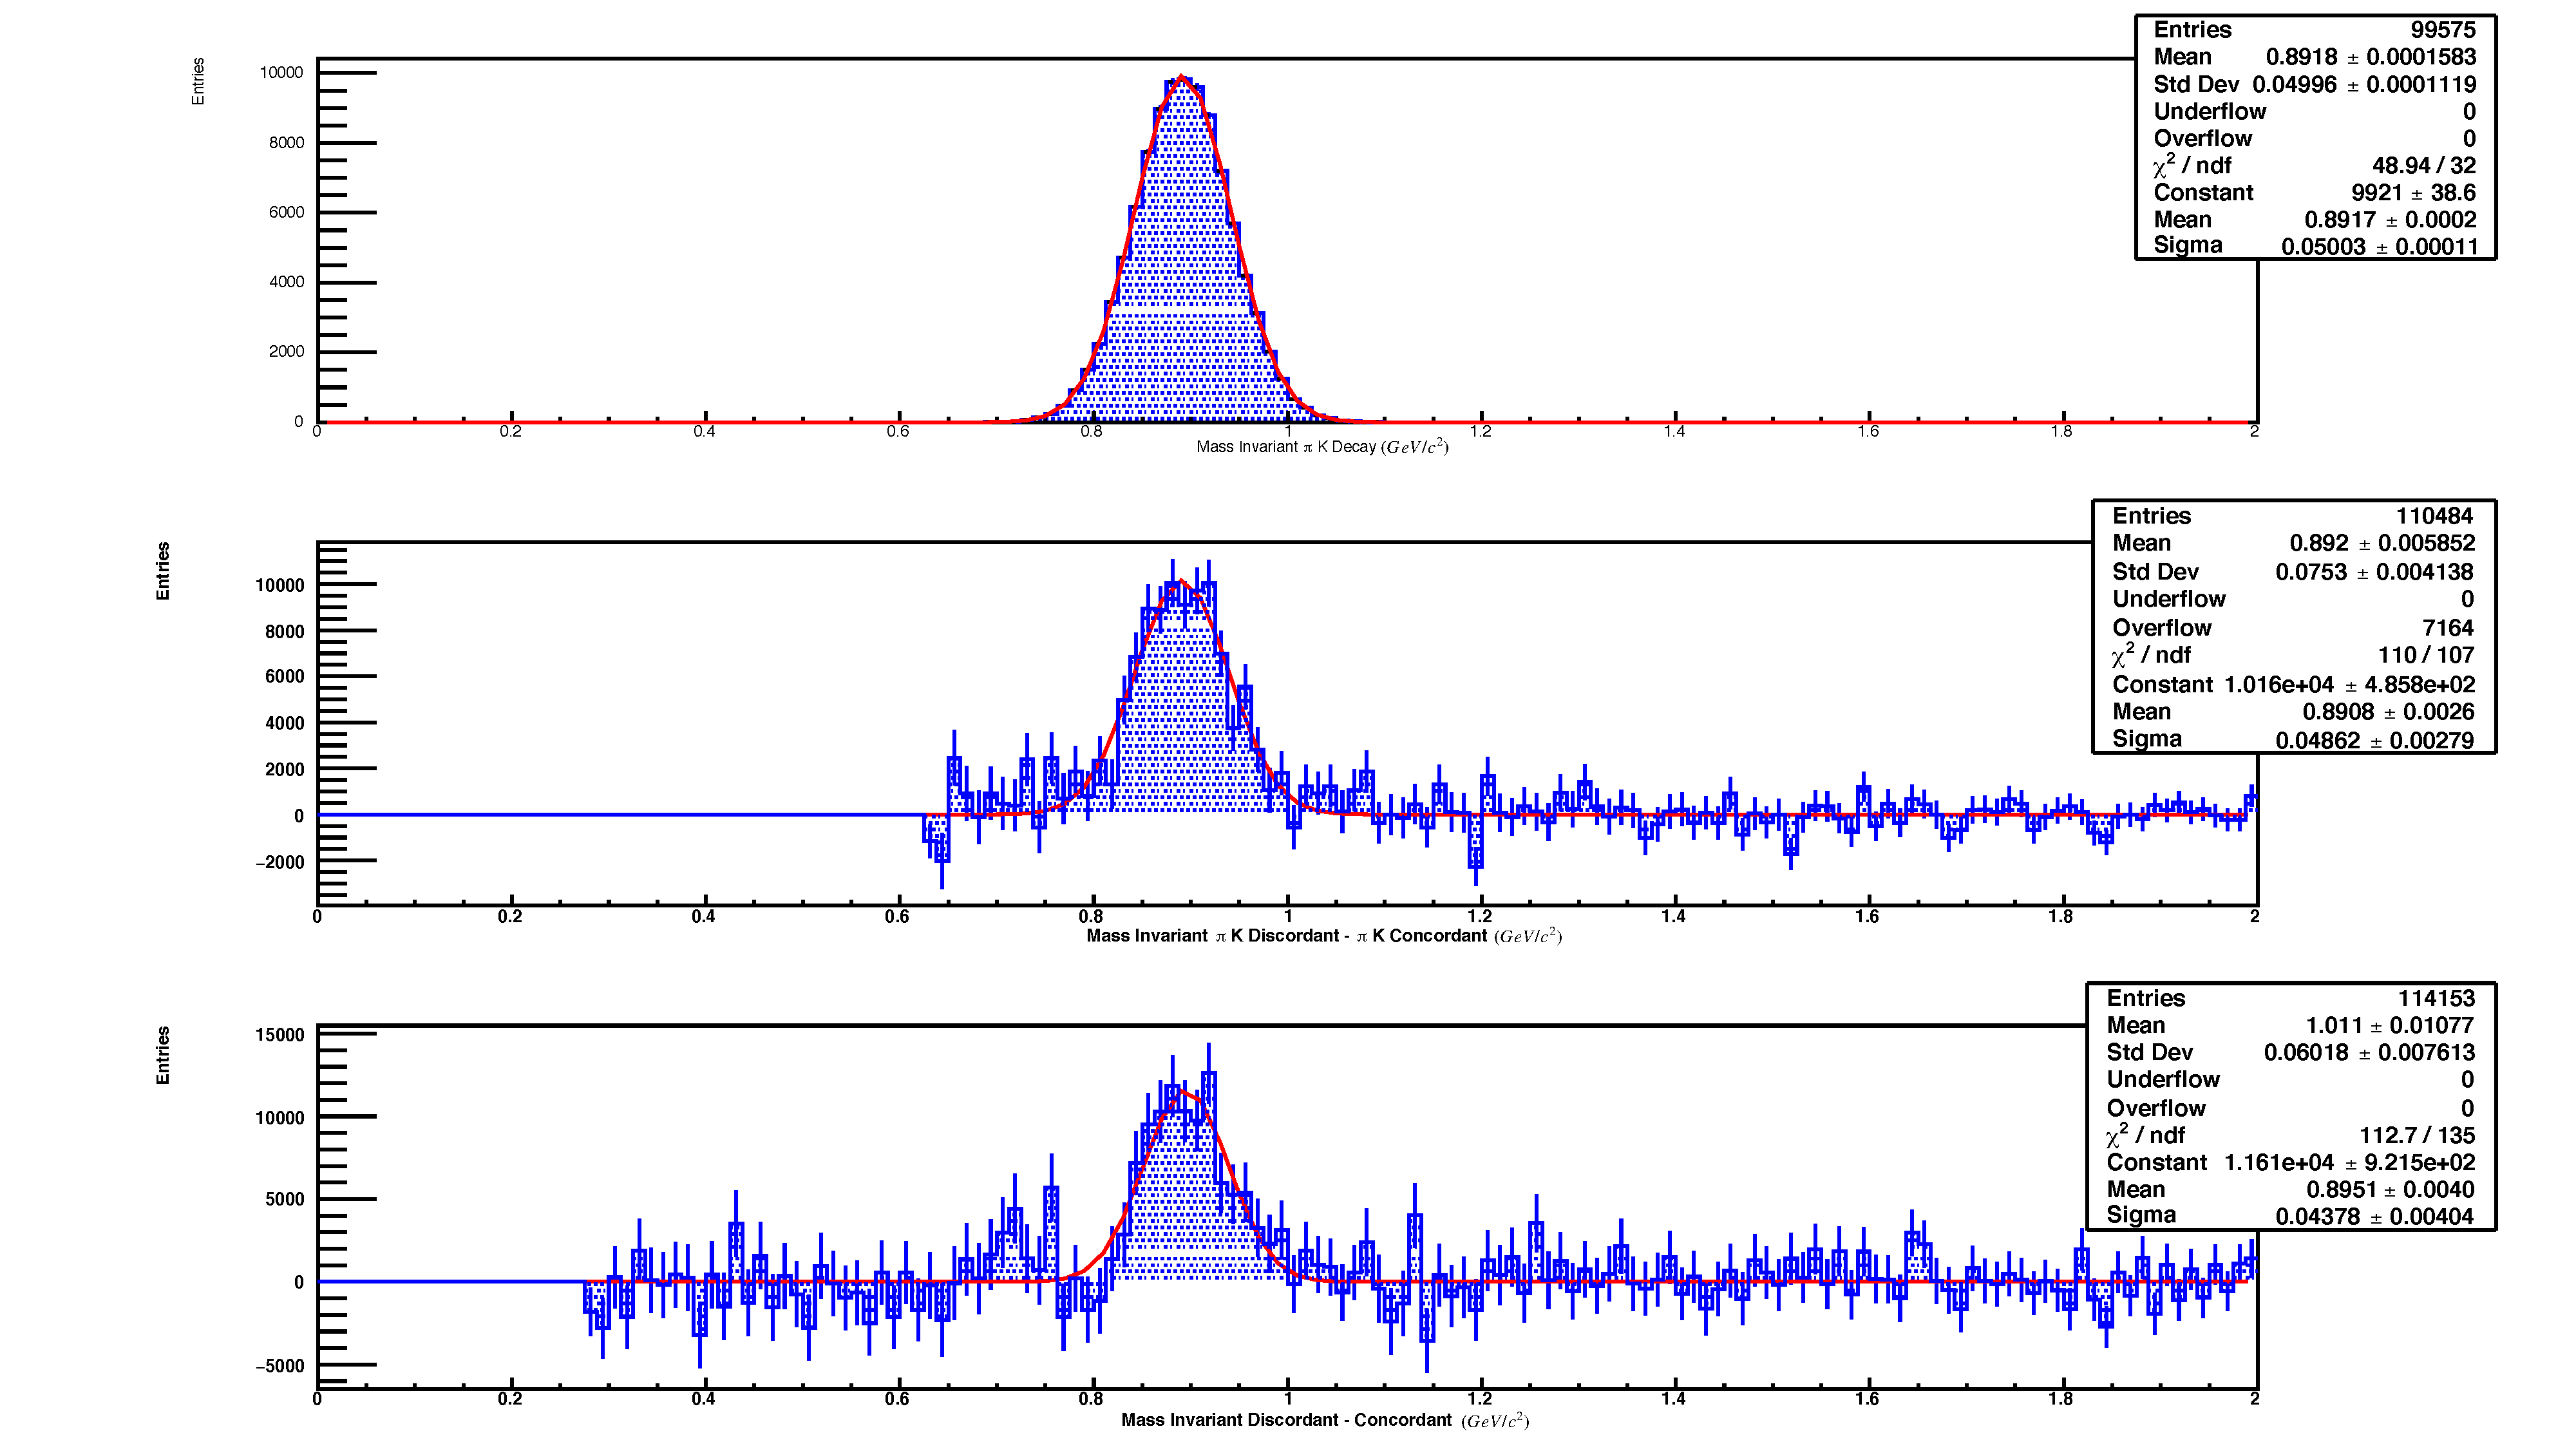
\includegraphics[scale=0.25]{c2.pdf}
    \caption{Il primo grafico dall'alto rappresenta l'istogramma delle masse invarianti delle $K^*$ vere, prodotte dal decadimento fittato con un'opportuna gaussiana;
    il secondo istogramma rappresenta la massa invariante ottenuta dalla differenza fra combinazioni $\pi$K di carica discorde e concorde anch'esso fittato con una gaussiana;
    il terzo istogramma rappresenta la massa invariante fra particella in combinazioni di carica discorde e concorde (fittato con un'opportuna gaussiana).}
\end{figure}

\section*{Appendice 1}
\subsection*{ParticleType.hpp}
\begin{lstlisting}
#ifndef PARTICLETYPE_HPP
#define PARTICLETYPE_HPP
#include <iostream>

class ParticleType {
protected:
  std::string const fName;
  double const fMass;
  int const fCharge;

public:
  ParticleType(std::string name, double mass, int charge);
  std::string getName();
  double getMass();
  int getCharge();
  virtual double getWidth();
  virtual void Print();
};

#endif
\end{lstlisting}

\subsection*{ParticleType.cpp}
\begin{lstlisting}
#include "ParticleType.hpp"

ParticleType::ParticleType(std::string name, double mass, int charge)
    : fName{name}, fMass{mass}, fCharge{charge} {}

std::string ParticleType::getName() { return fName; }

double ParticleType::getMass() { return fMass; }

int ParticleType::getCharge() { return fCharge; }

double ParticleType::getWidth() { return 0.; }

void ParticleType::Print() {
  std::cout << "Name: " << fName << '\n';
  std::cout << "Mass: " << fMass << '\n';
  std::cout << "Charge: " << fCharge << '\n';
  std::cout << '\n';
}
\end{lstlisting}

\subsection*{ResonanceType.hpp}
\begin{lstlisting}
#ifndef RESONANCETYPE_HPP
#define RESONANCETYPE_HPP

#include "ParticleType.hpp"

class ResonanceType : public ParticleType {
private:
  double const fWidth;

public:
  ResonanceType(ParticleType particle_t, double width);
  double getWidth() override;
  void Print() override;
};

#endif
\end{lstlisting}

\subsection*{ResonanceType.cpp}
\begin{lstlisting}
#include "ResonanceType.hpp"

ResonanceType::ResonanceType(ParticleType particle_t, double width)
    : ParticleType{particle_t}, fWidth{width} {}

double ResonanceType::getWidth() { return fWidth; }

void ResonanceType::Print() {
  std::cout << "Name: " << fName << '\n';
  std::cout << "Mass: " << fMass << '\n';
  std::cout << "Charge: " << fCharge << '\n';
  std::cout << "Resonance: " << fWidth << '\n';
  std::cout << '\n';
}
\end{lstlisting}

\subsection*{Particle.hpp}
\begin{lstlisting}
#ifndef PARTICLE_HPP
#define PARTICLE_HPP

#include "ParticleType.hpp"
#include "ResonanceType.hpp"
#include <algorithm>
#include <cmath>
#include <cstdlib>
#include <random>
#include <vector>

struct P {
  double fPx = 0;
  double fPy = 0;
  double fPz = 0;
};

class Particle {
private:
  static std::vector<ParticleType *> fParticleType;
  static int fNParticleType;
  int fIParticle;
  P fP;
  static int FindParticle(std::string name);
  void Boost(double bx, double by, double bz);

public:
  Particle(std::string name, P p);
  int getIParticle();
  static void AddParticle(std::string pt_name, double pt_mass, int pt_charge,
                          double pt_width);
  static void Print();
  void PrintParticle();
  P getP();
  std::string getName();
  double getMass();
  int getCharge();
  double Energy();
  double invMass(Particle &p);
  void setP(double px, double py, double pz);
  int Decay2Body(Particle &dau1, Particle &dau2);
};

#endif
\end{lstlisting}

\subsection*{Particle.cpp}
\begin{lstlisting}
#include "Particle.hpp"

std::vector<ParticleType *> Particle::fParticleType(1, nullptr);

int Particle::fNParticleType = 0;

int Particle::FindParticle(std::string name) {
  for (int i = 0; i != static_cast<int>(fParticleType.size()) - 1; ++i) {
    if (fParticleType[i]->getName() == name) {
      return i;
    }
  }
  return -1;
}

void Particle::Boost(double bx, double by, double bz) {
  double energy = Energy();

  double b2 = bx * bx + by * by + bz * bz;
  double gamma = 1.0 / std::sqrt(1.0 - b2);
  double bp = bx * fP.fPx + by * fP.fPy + bz * fP.fPz;
  double gamma2 = b2 > 0 ? (gamma - 1.0) / b2 : 0.0;

  fP.fPx += gamma2 * bp * bx + gamma * bx * energy;
  fP.fPy += gamma2 * bp * by + gamma * by * energy;
  fP.fPz += gamma2 * bp * bz + gamma * bz * energy;
}

Particle::Particle(std::string name, P p) : fP{p} {
  fIParticle = FindParticle(name);
}

int Particle::getIParticle() { return fIParticle; }

void Particle::AddParticle(std::string pt_name, double pt_mass, int pt_charge,
                           double pt_width) {
  ++fNParticleType;
  fParticleType[fNParticleType - 1] =
      new ParticleType{pt_name, pt_mass, pt_charge};
  if (pt_width != 0.) {
    fParticleType[fNParticleType - 1] =
        new ResonanceType{*fParticleType[fNParticleType - 1], pt_width};
  }
  fParticleType.push_back(nullptr);
}

void Particle::Print() {
  for (int i = 0; i != static_cast<int>(fParticleType.size()) - 1; ++i) {
    std::cout << "Name: " << fParticleType[i]->getName() << '\n';
    std::cout << "Mass: " << fParticleType[i]->getMass() << '\n';
    std::cout << "Charge: " << fParticleType[i]->getCharge() << '\n';
    std::cout << "Width: " << fParticleType[i]->getWidth() << "\n\n";
  }
}

void Particle::PrintParticle() {
  std::cout << "Index: " << fIParticle << '\n';
  std::cout << "Name: " << fParticleType[fIParticle]->getName() << '\n';
  std::cout << "Px: " << fP.fPx << '\n';
  std::cout << "Py: " << fP.fPy << '\n';
  std::cout << "Pz: " << fP.fPz << "\n\n";
}

P Particle::getP() { return fP; }

std::string Particle::getName() { return fParticleType[fIParticle]->getName(); }

double Particle::getMass() { return fParticleType[fIParticle]->getMass(); }

int Particle::getCharge() { return fParticleType[fIParticle]->getCharge(); }

double Particle::Energy() {
  double m = getMass();
  double p_x = fP.fPx;
  double p_y = fP.fPy;
  double p_z = fP.fPz;
  return std::sqrt((m * m) + (p_x * p_x) + (p_y * p_y) + (p_z * p_z));
}

double Particle::invMass(Particle &p) {
  double sumE = Energy() + p.Energy();

  double sumPx = getP().fPx + p.getP().fPx;
  double sumPy = getP().fPy + p.getP().fPy;
  double sumPz = getP().fPz + p.getP().fPz;

  return std::sqrt(sumE * sumE - sumPx * sumPx - sumPy * sumPy - sumPz * sumPz);
}

void Particle::setP(double px, double py, double pz) {
  fP.fPx = px;
  fP.fPy = py;
  fP.fPz = pz;
}

int Particle::Decay2Body(Particle &dau1, Particle &dau2) {
  if (getMass() == 0.0) {
    std::cout << "Decayment cannot be preformed if mass is zero\n";
    return 1;
  }

  double massMot = getMass();
  double massDau1 = dau1.getMass();
  double massDau2 = dau2.getMass();

  if (fIParticle > -1) {
    float x1, x2, w, y1, y2;

    double invnum = 1. / RAND_MAX;

    do {
      x1 = 2.0 * rand() * invnum - 1.0;
      x2 = 2.0 * rand() * invnum - 1.0;
      w = x1 * x1 + x2 * x2;
    } while (w >= 1.0);

    w = std::sqrt((-2.0 * std::log(w)) / w);
    y1 = x1 * w;
    y2 = x2 * w;
    massMot += fParticleType[fIParticle]->getWidth() * y1;
  }

  if (massMot < massDau1 + massDau2) {
    std::cout << "Decayment cannot be preformed because mass is too low in "
                 "this channel\n";
    return 2;
  }

  double pout =
      std::sqrt(
          (massMot * massMot - (massDau1 + massDau2) * (massDau1 + massDau2)) *
          (massMot * massMot - (massDau1 - massDau2) * (massDau1 - massDau2))) /
      massMot * 0.5;

  double norm = 2 * M_PI / RAND_MAX;

  double phi = rand() * norm;
  double theta = rand() * norm * 0.5 - M_PI / 2.;
  dau1.setP(pout * std::sin(theta) * std::cos(phi),
            pout * std::sin(theta) * std::sin(phi), pout * std::cos(theta));
  dau2.setP(-pout * std::sin(theta) * std::cos(phi),
            -pout * std::sin(theta) * std::sin(phi), -pout * std::cos(theta));

  double energy = std::sqrt(fP.fPx * fP.fPx + fP.fPy * fP.fPy +
                            fP.fPz * fP.fPz + massMot * massMot);

  double bx = fP.fPx / energy;
  double by = fP.fPy / energy;
  double bz = fP.fPz / energy;

  dau1.Boost(bx, by, bz);
  dau2.Boost(bx, by, bz);

  return 0;
}
\end{lstlisting}

\subsection*{main.cpp}
\begin{lstlisting}
// header file
#include "Particle.hpp"
#include "ParticleType.hpp"
#include "ResonanceType.hpp"

// ROOT's header file
#include "TFile.h"
#include "TH1.h"
#include "TH1F.h"
#include "TRandom.h"

int main() {
  using namespace std;

  Particle::AddParticle("pion+", 0.13957, 1, 0.);
  Particle::AddParticle("pion-", 0.13957, -1, 0.);

  Particle::AddParticle("kaon+", 0.49367, 1, 0.);
  Particle::AddParticle("kaon-", 0.49367, -1, 0.);

  Particle::AddParticle("proton+", 0.93827, 1, 0.);
  Particle::AddParticle("proton-", 0.93827, -1, 0.);

  Particle::AddParticle("K*", 0.89166, 0, 0.050);

  vector<Particle> particle_v{};

  TH1F *hPt = new TH1F("hPt", "Particle Types Distribution", 7, 0, 7);
  TH1F *hPhi = new TH1F("hPhi", "Phi Distribution", 100, 0., 2 * M_PI);
  TH1F *hTheta = new TH1F("hTheta", "Theta Distribution", 100, 0., M_PI);
  TH1F *hP = new TH1F("hP", "Momentum Distribution", 100, 0, 7);
  TH1F *hPtr = new TH1F("hPtr", "Trasversal Momentum Distribution", 80, 0, 5);
  TH1F *hE = new TH1F("hE", "Energy Distribution", 80, 0, 6);
  TH1F *hMass = new TH1F("hMass", "Mass Invariant Distribution", 320, 0, 4);
  TH1F *hMass_dc = new TH1F(
      "hMass_dc", "Mass Invariant Distribution with Discordant Charges", 160, 0,
      2);
  TH1F *hMass_sc = new TH1F(
      "hMass_sc", "Mass Invariant Distribution with Same Charges", 160, 0, 2);
  TH1F *hMass_pkD = new TH1F(
      "hMass_pkD", "Mass Invariant Distribution Pion+/Kaon- Pion-/Kaon+", 160,
      0, 2);
  TH1F *hMass_pkC = new TH1F(
      "hMass_pkC", "Mass Invariant Distribution Pion+/Kaon+ Pion-/Kaon-", 160,
      0, 2);
  TH1F *hMass_pkDecay = new TH1F(
      "hMass_pkDecay",
      "Mass Invariant Distribution Decay K* in Pion+/Kaon- Pion-/Kaon+", 160, 0,
      2);

  // Define random distributions using the random library
  random_device rd;
  mt19937 gen(rd());
  uniform_real_distribution<> distrib(0, 1);
  uniform_int_distribution<> int_distrib(0, 1);

  gRandom->SetSeed();

  for (int i = 0; i != 1e5; ++i) {
    for (int j = 0; j != 1e2; ++j) {
      int prob_type_decay = int_distrib(gen);
      double prob_type = distrib(gen);

      double phi = gRandom->Uniform(0., 2 * M_PI);
      hPhi->Fill(phi);

      double theta = gRandom->Uniform(0., M_PI);
      hTheta->Fill(theta);

      double p_ = gRandom->Exp(1);
      hP->Fill(p_);

      P linearMomentum;

      if (prob_type <= 0.4) {
        Particle pion{"pion+", linearMomentum};
        pion.setP(p_ * sin(theta) * cos(phi), p_ * sin(theta) * sin(phi),
                  p_ * cos(theta));
        particle_v.push_back(pion);
        hPt->Fill(pion.getIParticle());
        hPtr->Fill(sqrt(pow(p_ * sin(theta) * cos(phi), 2) +
                        pow(p_ * sin(theta) * sin(phi), 2)));
        hE->Fill(pion.Energy());
      }

      else if (prob_type > 0.4 && prob_type <= 0.8) {
        Particle pion_{"pion-", linearMomentum};
        pion_.setP(p_ * sin(theta) * cos(phi), p_ * sin(theta) * sin(phi),
                   p_ * cos(theta));
        particle_v.push_back(pion_);
        hPt->Fill(pion_.getIParticle());
        hPtr->Fill(sqrt(pow(p_ * sin(theta) * cos(phi), 2) +
                        pow(p_ * sin(theta) * sin(phi), 2)));
        hE->Fill(pion_.Energy());
      }

      else if (prob_type > 0.8 && prob_type <= 0.85) {
        Particle kaon{"kaon+", linearMomentum};
        kaon.setP(p_ * sin(theta) * cos(phi), p_ * sin(theta) * sin(phi),
                  p_ * cos(theta));
        particle_v.push_back(kaon);
        hPt->Fill(kaon.getIParticle());
        hPtr->Fill(sqrt(pow(p_ * sin(theta) * cos(phi), 2) +
                        pow(p_ * sin(theta) * sin(phi), 2)));
        hE->Fill(kaon.Energy());
      }

      else if (prob_type > 0.85 && prob_type <= 0.90) {
        Particle kaon_{"kaon-", linearMomentum};
        kaon_.setP(p_ * sin(theta) * cos(phi), p_ * sin(theta) * sin(phi),
                   p_ * cos(theta));
        particle_v.push_back(kaon_);
        hPt->Fill(kaon_.getIParticle());
        hPtr->Fill(sqrt(pow(p_ * sin(theta) * cos(phi), 2) +
                        pow(p_ * sin(theta) * sin(phi), 2)));
        hE->Fill(kaon_.Energy());
      }

      else if (prob_type > 0.9 && prob_type <= 0.945) {
        Particle proton{"proton+", linearMomentum};
        proton.setP(p_ * sin(theta) * cos(phi), p_ * sin(theta) * sin(phi),
                    p_ * cos(theta));
        particle_v.push_back(proton);
        hPt->Fill(proton.getIParticle());
        hPtr->Fill(sqrt(pow(p_ * sin(theta) * cos(phi), 2) +
                        pow(p_ * sin(theta) * sin(phi), 2)));
        hE->Fill(proton.Energy());
      }

      else if (prob_type > 0.945 && prob_type <= 0.99) {
        Particle proton_{"proton-", linearMomentum};
        proton_.setP(p_ * sin(theta) * cos(phi), p_ * sin(theta) * sin(phi),
                     p_ * cos(theta));
        particle_v.push_back(proton_);
        hPt->Fill(proton_.getIParticle());
        hPtr->Fill(sqrt(pow(p_ * sin(theta) * cos(phi), 2) +
                        pow(p_ * sin(theta) * sin(phi), 2)));
        hE->Fill(proton_.Energy());
      }

      else {
        Particle k_star{"K*", linearMomentum};
        k_star.setP(p_ * sin(theta) * cos(phi), p_ * sin(theta) * sin(phi),
                    p_ * cos(theta));
        particle_v.push_back(k_star);
        hPt->Fill(k_star.getIParticle());
        hPtr->Fill(sqrt(pow(p_ * sin(theta) * cos(phi), 2) +
                        pow(p_ * sin(theta) * sin(phi), 2)));
        hE->Fill(k_star.Energy());

        if (prob_type_decay != 0) {
          Particle pionD{"pion+", linearMomentum};
          Particle kaonD_{"kaon-", linearMomentum};
          k_star.Decay2Body(pionD, kaonD_);
          particle_v.push_back(pionD);
          particle_v.push_back(kaonD_);
          hMass_pkDecay->Fill(pionD.invMass(kaonD_));
        } else {
          Particle pionD_{"pion-", linearMomentum};
          Particle kaonD{"kaon+", linearMomentum};
          k_star.Decay2Body(pionD_, kaonD);
          particle_v.push_back(pionD_);
          particle_v.push_back(kaonD);
          hMass_pkDecay->Fill(pionD_.invMass(kaonD));
        }
      }
    }

    for (int i = 0; i != static_cast<int>(particle_v.size()); ++i) {
      for (int j = i + 1; j != static_cast<int>(particle_v.size()); ++j) {
        hMass->Fill(particle_v[i].invMass(particle_v[j]));

        if ((particle_v[i].getCharge() == 1 &&
             particle_v[j].getCharge() == 1) ||
            (particle_v[i].getCharge() == -1 &&
             particle_v[j].getCharge() == -1)) {
          hMass_sc->Fill(particle_v[i].invMass(particle_v[j]));
        } else if ((particle_v[i].getCharge() == 1 &&
                    particle_v[j].getCharge() == -1) ||
                   (particle_v[i].getCharge() == -1 &&
                    particle_v[j].getCharge() == 1)) {
          hMass_dc->Fill(particle_v[i].invMass(particle_v[j]));
        }

        if ((particle_v[i].getName() == "pion+" &&
             particle_v[j].getName() == "kaon-") ||
            (particle_v[i].getName() == "kaon-" &&
             particle_v[j].getName() == "pion+")) {
          hMass_pkD->Fill(particle_v[i].invMass(particle_v[j]));
        } else if ((particle_v[i].getName() == "pion-" &&
                    particle_v[j].getName() == "kaon+") ||
                   (particle_v[i].getName() == "kaon+" &&
                    particle_v[j].getName() == "pion-")) {
          hMass_pkD->Fill(particle_v[i].invMass(particle_v[j]));
        }

        if ((particle_v[i].getName() == "pion+" &&
             particle_v[j].getName() == "kaon+") ||
            (particle_v[i].getName() == "kaon+" &&
             particle_v[j].getName() == "pion+")) {
          hMass_pkC->Fill(particle_v[i].invMass(particle_v[j]));
        } else if ((particle_v[i].getName() == "pion-" &&
                    particle_v[j].getName() == "kaon-") ||
                   (particle_v[i].getName() == "kaon-" &&
                    particle_v[j].getName() == "pion-")) {
          hMass_pkC->Fill(particle_v[i].invMass(particle_v[j]));
        }
      }
    }
    particle_v.clear();
  }

  // Write Histograms into a ROOT file
  TFile *particle = new TFile("particle.root", "RECREATE");
  {
    particle->Write();
    hPt->Write();
    hPhi->Write();
    hTheta->Write();
    hP->Write();
    hPtr->Write();
    hE->Write();
    hMass->Write();
    hMass_dc->Write();
    hMass_sc->Write();
    hMass_pkD->Write();
    hMass_pkC->Write();
    hMass_pkDecay->Write();
    particle->Close();
  }
}
\end{lstlisting}

\subsection*{analysis.C}
\begin{lstlisting}
void setStyle() {
  // Cosmetics
  gROOT->SetStyle("Plain");
  gStyle->SetOptStat(112210);
  gStyle->SetOptFit(111);
  gStyle->SetOptTitle(0);
}

void analysis() {
  // Open Root File
  TFile *f = new TFile("particle.root");

  // Find Histograms
  auto hPt = (TH1F *)f->Get("hPt");
  auto hPhi = (TH1F *)f->Get("hPhi");
  auto hTheta = (TH1F *)f->Get("hTheta");
  auto hP = (TH1F *)f->Get("hP");
  auto hPtr = (TH1F *)f->Get("hPtr");
  auto hE = (TH1F *)f->Get("hE");
  auto hMass = (TH1F *)f->Get("hMass");
  auto hMass_dc = (TH1F *)f->Get("hMass_dc");
  auto hMass_sc = (TH1F *)f->Get("hMass_sc");
  auto hMass_pkD = (TH1F *)f->Get("hMass_pkD");
  auto hMass_pkC = (TH1F *)f->Get("hMass_pkC");
  auto hMass_pkDecay = (TH1F *)f->Get("hMass_pkDecay");

  TH1F *pkD_pkC = new TH1F("pkD_pkC",
                           "Difference between Pion+/Kaon- Pion-/Kaon+ Minus "
                           "Pion+/Kaon+ Pion-/Kaon-",
                           160, 0, 2);
  TH1F *dc_sc = new TH1F(
      "dc_sc", "Difference between Discordant Charges and Same Charges", 160, 0,
      2);

  // First Canvas
  TCanvas *c1 =
      new TCanvas("c1", "Particle Types, Angles and Momentum Distributioins",
                  100, 100, 1100, 700);
  {
    c1->Divide(2, 2);

    c1->cd(1);
    hPt->GetXaxis()->SetTitle("Types of Particles");
    hPt->GetYaxis()->SetTitle("Entries");
    hPt->GetXaxis()->CenterTitle();
    hPt->GetXaxis()->CenterTitle();
    hPt->SetLineColor(4);
    hPt->SetFillColor(4);
    hPt->SetFillStyle(3002);
    hPt->Draw("E");
    hPt->Draw("SAME");

    c1->cd(2);
    hPhi->GetXaxis()->SetTitle("Phi Angle");
    hPhi->GetYaxis()->SetTitle("Entries");
    hPhi->GetXaxis()->CenterTitle();
    hPhi->GetXaxis()->CenterTitle();
    hPhi->SetLineColor(4);
    hPhi->SetFillColor(4);
    hPhi->SetFillStyle(3002);
    hPhi->Fit("pol0");
    hPhi->Draw("E");
    hPhi->Draw("SAME");

    c1->cd(3);
    hTheta->GetXaxis()->SetTitle("Theta Angle");
    hTheta->GetYaxis()->SetTitle("Entries");
    hTheta->GetXaxis()->CenterTitle();
    hTheta->GetXaxis()->CenterTitle();
    hTheta->SetLineColor(4);
    hTheta->SetFillColor(4);
    hTheta->SetFillStyle(3002);
    hTheta->Fit("pol0");
    hTheta->Draw("E");
    hTheta->Draw("SAME");

    c1->cd(4);
    hP->GetXaxis()->SetTitle("Momentum");
    hP->GetYaxis()->SetTitle("Entries");
    hP->GetXaxis()->CenterTitle();
    hP->GetXaxis()->CenterTitle();
    hP->SetLineColor(4);
    hP->SetFillColor(4);
    hP->SetFillStyle(3002);
    hP->Fit("expo");
    hP->Draw("E");
    hP->Draw("SAME");

    c1->Print("c1.gif");
  }

  // Second Canvas
  TCanvas *c2 = new TCanvas("c2", "Mass Invariant", 400, 100, 1100, 700);
  {
    c2->Divide(1, 3);

    c2->cd(1);
    hMass_pkDecay->GetXaxis()->SetTitle("Mass Invariant #pi K Decay");
    hMass_pkDecay->GetYaxis()->SetTitle("Entries");
    hMass_pkDecay->GetXaxis()->CenterTitle();
    hMass_pkDecay->GetXaxis()->CenterTitle();
    hMass_pkDecay->SetLineColor(4);
    hMass_pkDecay->SetFillColor(4);
    hMass_pkDecay->SetFillStyle(3002);
    hMass_pkDecay->Fit("gaus");
    hMass_pkDecay->Draw("E, SAME");

    c2->cd(2);
    pkD_pkC->GetXaxis()->SetTitle(
        "Mass Invariant #pi K Discordant - #pi K Concordant");
    pkD_pkC->GetYaxis()->SetTitle("Entries");
    pkD_pkC->GetXaxis()->CenterTitle();
    pkD_pkC->GetXaxis()->CenterTitle();
    pkD_pkC->SetLineColor(4);
    pkD_pkC->SetFillColor(4);
    pkD_pkC->SetFillStyle(3002);
    pkD_pkC->Sumw2();
    pkD_pkC->Add(hMass_pkD, hMass_pkC, 1, -1);
    pkD_pkC->SetEntries(pkD_pkC->Integral());
    pkD_pkC->Fit("gaus");
    pkD_pkC->Draw("HIST, SAME");

    c2->cd(3);
    dc_sc->GetXaxis()->SetTitle("Mass Invariant Discordant - Concordant");
    dc_sc->GetYaxis()->SetTitle("Entries");
    dc_sc->GetXaxis()->CenterTitle();
    dc_sc->GetXaxis()->CenterTitle();
    dc_sc->SetLineColor(4);
    dc_sc->SetFillColor(4);
    dc_sc->SetFillStyle(3002);
    dc_sc->Sumw2();
    dc_sc->Add(hMass_dc, hMass_sc, 1, -1);
    dc_sc->SetEntries(dc_sc->Integral());
    dc_sc->Fit("gaus");
    dc_sc->Draw("HIST, SAME");

    c2->Print("c2.gif");
  }
}
\end{lstlisting}
\end{document}
